\chapter{Korrespondance Analyse} \label{sec:Kor}
Korrespondance problemet, imellem to eller flere billeder af samme objekt eller scene, referere til problemet om at finde et sæt af punkter i det ene billede, der kan identificeres i det andet.
Udfordringen ved problemet ligger i at billederne, der skal matches, er udsat for en række ændringer, det kan f.eks. være forskydning i kameraets position ift. scenen eller  ændringer i scenens motiv.
 Et godt eksempel på korrespondance problemet er det menneskelige syn. Øjnene agere som to kameraer, der hver især fanger deres billede og omdanner disse billeder til et sammenhængende panoramisk billede, ved hjælp af oprettelse af korrespondancer. 
Korrespondancen mellem tillader også mennesket at opfatte dybde, hvilket skyldes den horisontale forskydning af menneskets øjne. Denne sektion vil beskrive, hvordan denne korrespondance  kan efterlignes af en computer
 
\begin{figure}[H]
    \centering
    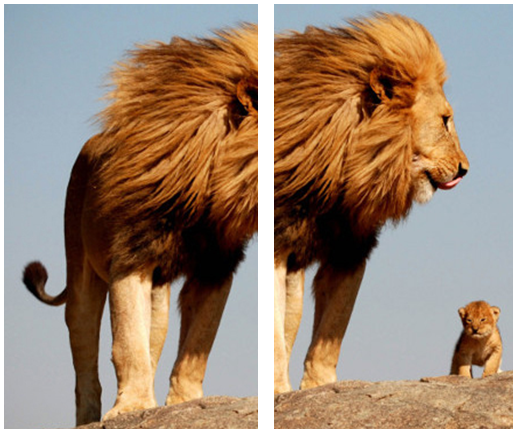
\includegraphics[width=0.55\textwidth]{fig/3.png}
    \begin{center}    
    \caption{
     De to ovenstående billeder er af samme 2-D motiv, med kamerapositionen forskudt i x-aksen.}
    \label{fig:1}
     \end{center}
  \end{figure}
I figur \ref{fig:1} ses to billeder af det samme motiv, men hvor kameravinklen er forskudt. For at opnå korrespondance imellem billederne skal der detekteres nogle unikke punkter, som skal optræde i begge billeder, dvs. der hvor billederne overlapper. Punkterne skal nøje beskrives så de kan genkendes i transformerede billeder. Til sidst skal punkterne matches for at estimere hvordan de korrespondere med hinanden, altså i dette tilfælde, hvordan de er forskudt i forhold til hinanden. Korrespondance analysens pipeline, der består af feature detektion, deskription og matching, er yderligere beskrevet i dette afsnit.
\section{Detektor}
Feature detektion er en metode indenfor billedbehandling, der determinere for hvert punkt i et billede, om dette punkt er et interessepunkt, altså om punktet kan anvendes i oprettelsen af korrespondancer. Detektorens resultat vil derved være et subset af isolerede punkter fra billedet, der er markeret som interessante eller distinktive. (Så hvornår er punkter interessante?) Der er ikke nogen klar definition for hvad der udgør et interessepunkt, men defineres ofte ift. hvilket applikationsdomæne detektoren indgår i. Uanset hvordan punkter udvælges, er målet at punkterne er repeterbare i begge billeder, dvs. punkter, der udvælges af detektoren i det ene billede, skal også udvælges i det andet af samme detektor. Detektionen skal derved være stabilt, men også robust ift. ændringer i billederne. Den udvalgte metode skal derfor være i stand til at udvælge repeterbare genkendelige områder i begge billeder, hvor disse områder er defineret ift. metoden der anvendes.  Udvælges punkterne ikke konsistent i begge billeder, er korrespondance oprettelsen ikke mulig. Korrespondance analysen er derved kun så god som feature detektoren. 
Interesse punkter defineres ikke udefra semantiske meningsfulde områder som ansigter eller andre menneske fortfolkelige objekter, men derimod pixel områder, der er matematisk distinktive. Som nævnt er dissse metoder ofte applikationsspecifikke og dikteret af hvilke objekter der forekommer i scenen. \\

Denne sektion vil beskrive, i detaljer, hvordan interessepunkter kan formuleres matematisk ift. de forskellige metoder.
<hvad er en god feature>
<corner>
<blob>
<edge>
\section{Deskriptor}
<Invariant>
\section{Matching}
